%%%%%%%%%%%%%%%%%%%%%%%%%%%%%%%%%%%%%%%%%
% FRI Data Science_report LaTeX Template
% Version 1.0 (28/1/2020)
%
% Jure Demšar (jure.demsar@fri.uni-lj.si)
%%%%%%%%%%%%%%%%%%%%%%%%%%%%%%%%%%%%%%%%%

%----------------------------------------------------------------------------------------
%   PACKAGES AND OTHER DOCUMENT CONFIGURATIONS
%----------------------------------------------------------------------------------------
\documentclass[fleqn,moreauthors,10pt]{ds_report}
\usepackage[english]{babel}

\graphicspath{{fig/}}

%----------------------------------------------------------------------------------------
%   ARTICLE INFORMATION
%----------------------------------------------------------------------------------------

\JournalInfo{Machine Learning for Data Science 1, 2025-2026}
\Archive{Homework 5 Report}
\PaperTitle{Kernels: Kernelized Ridge Regression and SVR}
\Authors{Denis Nedić}
\affiliation{\textit{dn98183@student.uni-lj.si}}

%----------------------------------------------------------------------------------------

\makeatletter
\renewcommand{\@maketitle}{%
\twocolumn[{%
\thispagestyle{empty}%
{
\includegraphics[height=2cm]{logo}}
\vskip-74pt%
{\raggedleft\small\sffamily\bfseries\@JournalInfo\\\@Archive\par}%
\vskip64pt%
{\raggedright\color{color1}\fontfamily{cmss}\fontseries{bc}\fontshape{n}\fontsize{20}{25}\selectfont \@PaperTitle\par}%
\vskip10pt%
{\raggedright\color{color1}\sffamily\fontsize{12}{16}\selectfont  \@Authors\par}%
\vskip8pt%
\begingroup%
\raggedright\sffamily\small%
\footnotesize\@affiliation\par%
\endgroup%
\vskip10pt%
}]%
}
\makeatother

\begin{document}

\flushbottom
\maketitle
\thispagestyle{empty}

%----------------------------------------------------------------------------------------
%   ARTICLE CONTENTS
%----------------------------------------------------------------------------------------

\section*{Introduction}
I implemented two kernels, polynomial $k(x,x')=(x\cdot x' + 1)^M$ and RBF
$k(x,x')=\exp(-\|x-x'\|^2/(2\sigma^2))$, and two regression methods: kernelized
ridge regression (KRR) and $\varepsilon$-insensitive support vector regression
(SVR). Both methods are illustrated on the 1D sine dataset and then
evaluated systematically on housing2r, where I compare them across kernels
and parameter settings.

%------------------------------------------------

\section*{Implementation}

\textbf{1. Kernels.}\\
Both kernels are implemented as callable classes that accept any combination of
1D and 2D inputs and return the appropriate scalar, vector, or matrix. The RBF
kernel computes pairwise squared distances via the polarisation identity
$\|x-x'\|^2 = \|x\|^2 + \|x'\|^2 - 2x\cdot x'$, so the implementation is fully
vectorised with no Python loops.
\vspace{0.3cm}
\\
\textbf{2. KRR.}\\
Kernelized ridge regression has a closed-form dual solution
$\alpha = (K + \lambda I)^{-1}y$, solved with a single linear-system solve.
Predictions on new inputs are $\hat{y} = K_{\text{test}}\alpha$. This is one
matrix factorisation and it is the same for any kernel.
\vspace{0.3cm}
\\
\textbf{3. SVR as a quadratic program.}\\
SVR cannot be solved in closed form, because its objective combines a squared
term with linear inequality constraints (the $\varepsilon$-tube and slack
penalties). The standard recipe is to dualise the problem, giving a quadratic
objective in $2n$ unknowns (one $\alpha_k$ and one $\alpha_k^*$ per training
point) subject to linear box constraints and one linear equality -- exactly
Eq.~(10) of Smola \& Schölkopf (2004).

I solved this with the cvxopt QP solver, which expects the problem in
standard form: minimise a quadratic in a vector of unknowns subject to linear
inequalities and equalities. My fit function builds the matrices that
describe Eq.~(10) in this form. The $2n$ unknowns are ordered as
$[\alpha_1,\alpha_1^*,\alpha_2,\alpha_2^*,\dots]$, which lets me build the
quadratic-term matrix as a Kronecker product between the kernel matrix and a
fixed $2\!\times\!2$ sign pattern. I also symmetrise the kernel matrix and
add a tiny diagonal jitter ($10^{-10}$) so the solver's factorisation stays
stable when the kernel matrix is nearly rank-deficient -- a real issue at
high polynomial degrees. Prediction weights are
$\beta_k = \alpha_k - \alpha_k^*$, and the bias $b$ is read directly from
cvxopt's equality-constraint multiplier rather than from Eq.~(16) of the
paper (which is numerically sensitive and contains an error).

%------------------------------------------------

\section*{Part 1: Fits on the sine Dataset}

The input $x$ was standardised before fitting, since the polynomial kernel
$(x\cdot x'+1)^M$ explodes on the raw scale; predictions are plotted against
the original $x$. Hand-tuned settings: $M=12$ with $\lambda=10^{-5}$ for the
polynomial kernel and $\sigma=0.2$ (in standardised units) with
$\lambda=10^{-3}$ for the RBF kernel. For SVR I used $\varepsilon=0.4$, which
is roughly the noise scale of the data and yields a sparse solution with 41
support vectors out of 200 training points. Figure~\ref{fig:sine} shows that
all four combinations track the underlying sinusoid closely (train MSE
0.07--0.08), with KRR fits slightly smoother and SVR fits keeping most points
inside the $\pm\varepsilon$ tube.

\begin{figure}[h!]
    \centering
    
\includegraphics[width=\columnwidth]{part1_sine.png}
    \caption{KRR and SVR on sine with polynomial ($M=12$) and RBF
    ($\sigma=0.2$) kernels. The dashed lines mark the $\pm\varepsilon$ tube.}
    \label{fig:sine}
\end{figure}

The fits at the right boundary show the inductive bias of the two kernels
clearly: the polynomial fit extrapolates aggressively upward (toward
$y\!\approx\!8$ just past the data), while the RBF fit decays back toward the
local mean once outside the support. Inside the data the two are almost
indistinguishable.

%------------------------------------------------

\section*{Part 2: Evaluation on housing2r}

\textbf{1. Setup.}\\
I held out 20\% of the 200-sample dataset (40 test, 160 train) and standardised
features using training statistics only. For each kernel-parameter value I
report two test MSEs: with $\lambda$ fixed at $1$ and with $\lambda$ selected
by 5-fold internal cross-validation on the training set over a log-spaced grid
$\lambda \in \{10^{-3},\dots,10^{3}\}$ (13 values). The model is then refit on
the full training set with the chosen $\lambda$ and evaluated on the held-out
test set.

For SVR I set $\varepsilon=2$. The training target has $\sigma_y\!\approx\!8.2$,
so this is a tube of about $\tfrac{1}{4}\sigma_y$ around predictions, wide
enough that many points fall inside (and contribute no SVs) but narrow enough
to fit well. A sensitivity analysis below confirms this is reasonable.

\textit{Baselines.} Predicting the training mean gives test MSE $44.2$, and
ordinary linear regression gives test MSE $19.4$. Everything below should be
compared against these.
\vspace{0.3cm}
\\
\textbf{2. Sweep results.}\\
Figure~\ref{fig:housing} shows test MSE and SV count as functions of the kernel
parameter for both methods.

\begin{figure}[h!]
    \centering
    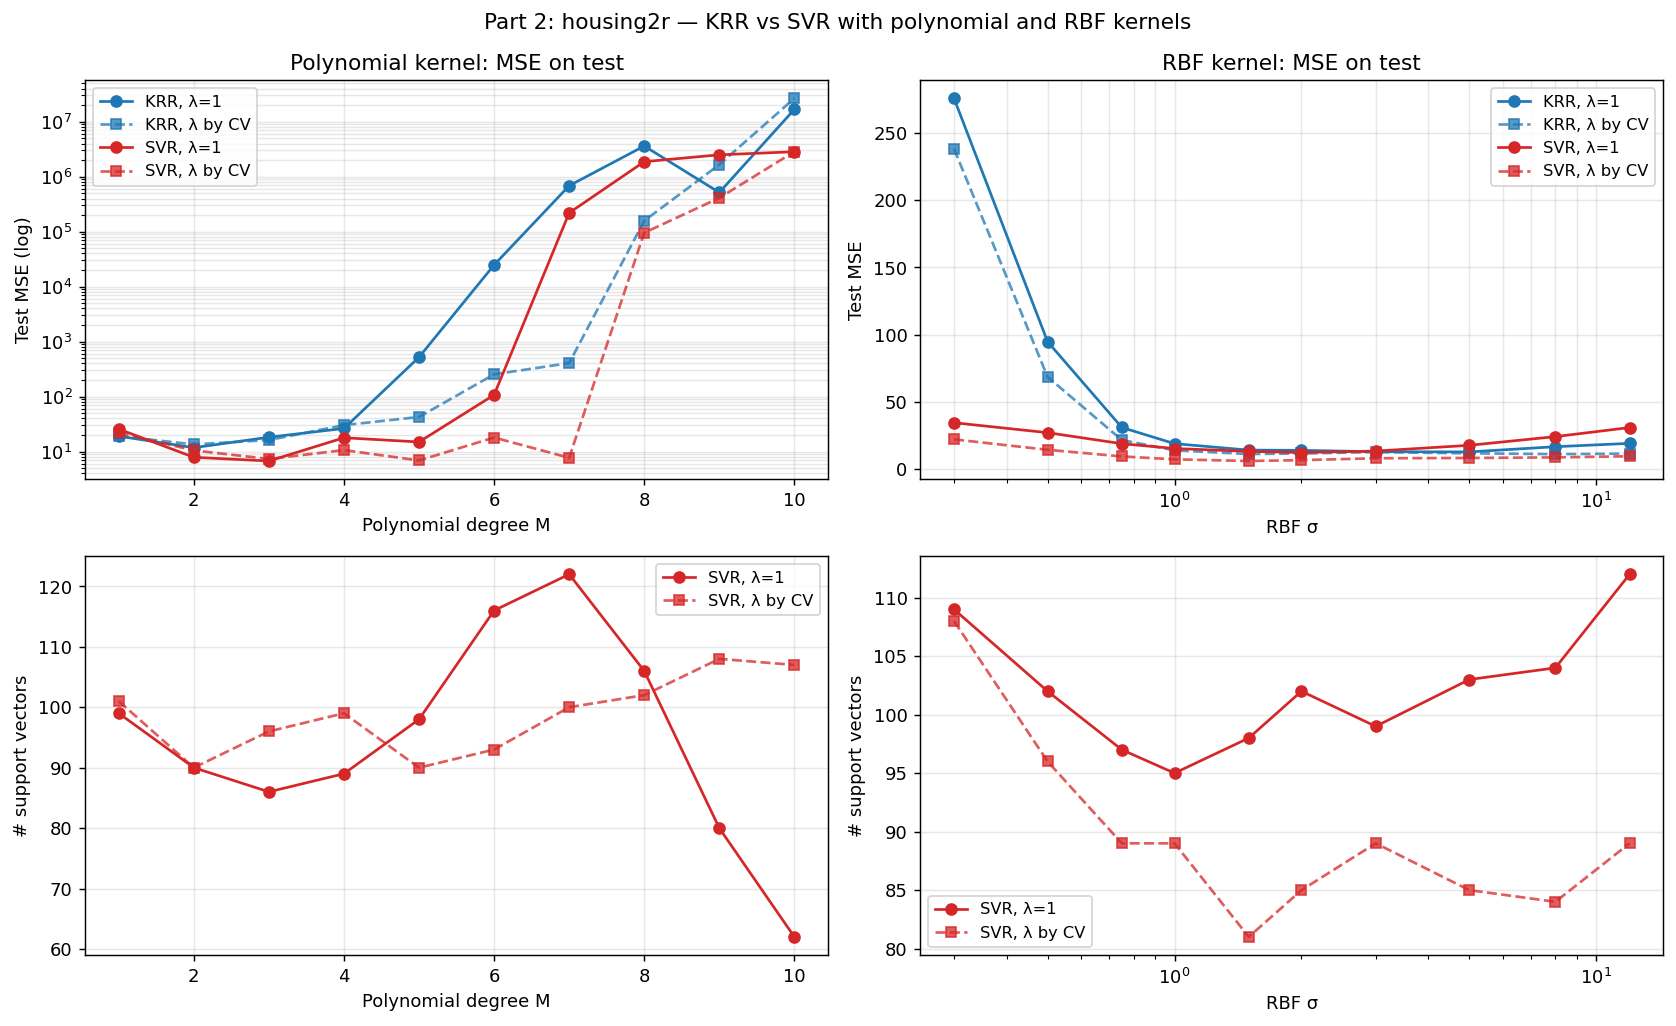
\includegraphics[width=\columnwidth]{part2_housing2r.png}
    \caption{Top: test MSE versus kernel parameter. Bottom: SVR support-vector
    counts. Polynomial MSE is plotted on a log scale because the values span
    seven orders of magnitude.}
    \label{fig:housing}
\end{figure}

For the polynomial kernel, both methods do well up to $M\!=\!3$ and then
diverge dramatically. KRR with $\lambda=1$ reaches MSE $> 10^7$ at $M=10$,
and even CV-tuned KRR with $\lambda=1000$ cannot stabilise it: the kernel
entries $(x\cdot x'+1)^M$ grow combinatorially with $M$ in five dimensions,
and the kernel matrix becomes badly ill-conditioned. SVR degrades much more
gracefully -- through $M=5$ it stays at MSE $\sim 7$--$15$ with CV -- because
its box constraint caps how much any single training point can contribute to
the prediction.

For the RBF kernel, behaviour is much better for both methods, with a broad
valley around $\sigma\in[1,3]$. KRR-CV bottoms out near MSE $11.2$ at
$\sigma=8$ (with $\lambda\!\approx\!0.03$), while SVR-CV reaches MSE $6.1$ at
$\sigma=1.5$ with about half of training points as support vectors.

\textit{A note on the SV plot.} For SVR with $\lambda=1$ and polynomial
$M=10$, the SV count drops to $62$, lower than at any other $M$. This is not
useful sparsity: the fit has collapsed (MSE $> 10^6$), so most points land
inside a hugely wide tube around a useless prediction. Low SV count is
informative only when paired with low MSE.
\vspace{0.3cm}
\\
\textbf{3. Epsilon sensitivity.}\\
To justify $\varepsilon=2$ and show the sparsity--fit tradeoff, I swept
$\varepsilon$ on a fixed good operating point (RBF $\sigma=1.5$, $\lambda=1$).
Figure~\ref{fig:eps} shows the result.
 
\begin{figure}[h!]
    \centering
    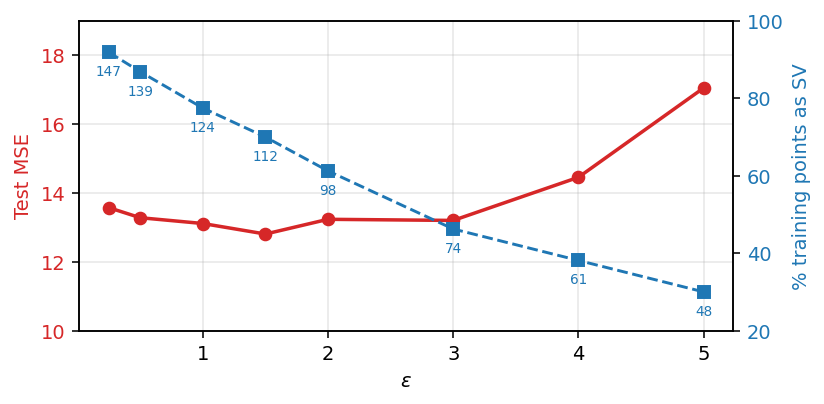
\includegraphics[width=\columnwidth]{epsilon_sweep.png}
    \caption{Test MSE (left axis, red) and number of support vectors
    (right axis, blue) versus $\varepsilon$ at RBF $\sigma=1.5$, $\lambda=1$.
    Raw SV counts are annotated on the blue curve.}
    \label{fig:eps}
\end{figure}
 
MSE is essentially flat from $\varepsilon=0.25$ to $\varepsilon=3$
(13.6 down to 13.0), while the SV count drops monotonically from
$147$ (92\% of training points) to $74$ (46\%). Beyond $\varepsilon=3$
MSE starts climbing. At $\lambda=1$ the knee at $\varepsilon\!\approx\!3$
looks optimal, but re-running the full sweep with $\varepsilon=3$ shows
the RBF results get worse under CV-tuned $\lambda$ (best MSE rises from
$6.1$ to $7.3$), while the polynomial results improve slightly. The
reason is that CV selects $\lambda\!\approx\!0.03$ for RBF, and with
that regularisation a tube of $\varepsilon=3$ is too wide. It
excludes too many training points. This shows that $\varepsilon$ and
$\lambda$ interact: $\varepsilon=2$ was retained as it gives the best
overall result under CV.
\vspace{0.3cm}
\\
\textbf{4. Best-setting comparison.}\\
Table~\ref{tab:best} summarises the best CV-tuned result for each
(method, kernel) combination.
 
\begin{table}[h!]
    \centering
    \caption{Best CV-tuned test MSE per method/kernel on housing2r.}
    \vspace{0.1cm}
    \label{tab:best}
    \resizebox{\columnwidth}{!}{%
    \begin{tabular}{llccc}
        \hline
        \textbf{Method} & \textbf{Kernel} & \textbf{Best param} & \textbf{MSE} & \textbf{\#SV} \\
        \hline
        KRR & Polynomial & $M=2$            & 13.5 & --  \\
        KRR & RBF        & $\sigma=8$       & 11.2 & --  \\
        SVR & Polynomial & $M=5$            & 6.9  & 90  \\
        SVR & RBF        & $\sigma=1.5$     & \textbf{6.1} & 81 \\
        \hline
        Linear regression & --- & --- & 19.4 & --- \\
        \hline
    \end{tabular}%
    }
    \vspace{0.1cm}
\end{table}


%------------------------------------------------

\section*{Conclusion}

I would prefer SVR. It is much more robust than KRR in the polynomial sweep
(KRR cannot cope with ill-conditioned kernel matrices, while SVR's box
constraint keeps any one point from dominating), gives the lowest overall MSE
($6.1$, vs.\ $11.2$ for KRR and $19.4$ for linear regression), and is sparse.

\end{document}